The phase field method, rooted in system thermodynamics, offers a solution for an interface with a finite thickness, an idea originating from van der Waals in 1893 \cite{vanderwaals1979ThermodynamicTheoryCapillarity}. This method models the free energy of the system and can derive a phase field method for interfacial dynamics. It offers several advantages, such as mass conservation, contact line motion, and adherence to thermodynamic laws. In contrast to the hydrodynamic theory, the contact line moves through interfacial diffusion. However, there are concerns about its validity in modeling macroscopic contact line motion, especially regarding the sharp-interface limit. Despite these concerns, meaningful results have been predicted on the macro scale that align with hydrodynamic theory and experimental observations\cite{yue2010SharpinterfaceLimitCahn,yue2011CanDiffuseinterfaceModels,carlson2011DissipationRapidDynamic}.


Phase field simulations for macroscopic wetting typically rely on the Cahn-Hilliard equations. For slow wetting phenomena, the phase field theory has been both analytically \cite{jacqmin2000ContactlineDynamicsDiffuse} and numerically \cite{yue2011CanDiffuseinterfaceModels,yue2010SharpinterfaceLimitCahn} proven to capture such wetting physics. However, for rapid spreading of water drops, the assumption of local equilibrium may not hold. Some studies have introduced a boundary condition for wetting far from equilibrium, introducing a parameter that controls the relaxation towards equilibrium . This parameter has been interpreted in various ways, from a local friction adjacent to the contact line to a relaxation parameter at the contact line\cite{yue2011WallEnergyRelaxation}\cite{carlsonCapillarityDynamicWetting2012}.


\paragraph{Phase Field Theory}
Die Phasenfeld theorie verwendet Ansätze beider Modelle unter verwendung der Beschreibung der freien Energie des Systems.\todo{ref chapter PhaseField}

Daher ist es auch notwendig für die Phasenfeldmethode sowohl hydrodynamische Ansätze als auch Ansätze der Molekular Kinetik Theorie zu verwenden \cite{blake2006PhysicsMovingWetting, carlsonCapillarityDynamicWetting2012}.

vof and level setzt
difference interface tracking and capituring? 

Free energy system 




\todo[inline]{einleitende Worte}

Wie bereits in Kapitel \ref{sec: Wetting_SurfaceTension} beshcrieben, gibt es unterschiedliche Möglichkeiten das Interface zu beschreiben. Hydrodynamische Modelle beschreiben das Interface so, dass am Übergang der Phasen die Stoffwerte springen. Ein Diffuses Interface hingegen, beschreibt die größen anders. \todo{picture of interfaces}

\section{Phase Field Method in the Spirit of Cahn and Hillard}
Die Phasenfeld Methode geht zurück auf die Idee von van der Waals \cite{vanderwaals1979ThermodynamicTheoryCapillarity}, der das Interface zwischen zwei nicht mischbaren Fluiden aus Sicht der Thermodynamik beschrieben hat. Darin gehen die Material Eigenschaften kontinuierlich innerhalb einer dünnen Schicht ineinander über. Innerhalb dieser Schicht existieren beide Phasen. 
Darauf aufbauend haben Cahn und Hillard \cite{johnw.FreeEnergyNonuniform1958} eine Beschreibung der freien Energie in einem Volumen mit ungleicher Zusammensetzung in Abhängigkeit eines Ordnungsparameters $C$ für Zeitabhängige Probleme abgeleitet. In geschlossener Form lautet diese
\begin{equation}
\label{eq: CahnHillard}
    \partial C + \textbf{u} \cdot \nabla C = \nabla \cdot \left(\kappa \nabla \phi(C)\right).
\end{equation}
Darin ist $\textbf{u}$ die Geschwindigkeit, $\kappa$ ein Diffusionskoeffizient, meist mobility genannt, und $\phi$ ein chemisches Potential. Der ordnungsparameter gibt an welche phase vorliegt und liegt für ein zwei phasen system zwischen $-1$ und $1$. Die Mobilität kann mit der Péclet Zahl in Verbindung gebracht werden, die eine Verhältnis der advektiven zu diffusiven flüssen mit einer charakteristischen Weglänge ($L_{char}$) und Geschwindigkeit ($u_{char}$), sowie einem Charakterischen chemischen Potential abbildet\cite{cai2015NumericalSimulationWetting,holzinger2021DirectNumericalSimulation}. 
Das chemische Potential ist als Ableitung der freien Helmholz Energie bezüglich des Ordungsparameters definiert \cite{johnw.FreeEnergyNonuniform1958}. Im behandelten System kann setzt sich die gesamte freie Energie aus der Mischungsenergie und der interfacial density energy zusammen. Nach \cite{yue2010SharpinterfaceLimitCahn} ist die freie Energie des Systems durch zwei Einflüsse gegeben; definiert über das Volumen $\Omega$ und die Oberfläche $\partial\Omega$ \todo{check!!!}
\begin{equation}
    F(C, \nabla C) = \int_{\Omega} f_{\mathrm{mix}} (C, \nabla C) d\textbf{x}+ \int_{\partial\Omega}f_\mathrm{w}(C) dS
\end{equation}
Darin ist das erste integral das der mischungsenergiedichte $f_{mix}$ und das zweite der Wand $f_w$.

\subsection{Mixing Energy}
Cahn und Hillard haben eine mischungsenergie ($f_{mix}$) definiert, die vom Ordnungsparameter und seinem Gradienten abhängt:
\begin{equation}
    F(C, \nabla C) = \int_{\Omega} f_{\mathrm{mix}} (C, \nabla C) d\textbf{x} = \int_{\Omega}\left(\frac{\lambda}{\epsilon^2}\Psi(C)+\frac{\lambda}{2}\vert\nabla C\vert^2\right)d\textbf{x}
\end{equation}\todo{check if right function}
Die integration der Mischungsenergie über den Bereich ergibt die freie Helmholz Energie des Fluidsystems und besteht aus zwei Summanden. Der erste Term trennt die Phasen voneinander ab, während der zweite Term die Phasen mischt. $\lambda$ ist ein mischungsenergie Parameter, $\epsilon$ ein maß für die Dicke des Interfaces\todo{check if already mentioned} und $\Psi$ ein Potential. Das Potential wird nach Ginzburg und Landau\todo{cite} so gewählt, dass es zwei Minima an den stellen $-1$ und $1$ hat und ist gegeben mit 
\begin{equation}
    \Psi(C)= \frac{1}{4}\left(C^2-1\right)^2.
\end{equation}
Daraus folgt die folgende Darstellung für das chemische Potential 
\begin{equation}
    \label{eq: chempotentialMIXING_pahseFieldMethod}
    \Phi(C):= \frac{\partial F(C)}{\partial C} = \frac{\lambda}{\epsilon^2}\Psi'(C)-\lambda\nabla^2C.
\end{equation}


\subsection{Diffusive Interaface}
Das Cahn Hillard Modell kann Systeme mit mehreren Fluiden beschreiben. In dieser Arbeit wird jedoch nur ein binäres Fluidsystem betrachtet. 
\begin{figure}[h]
    \centering
    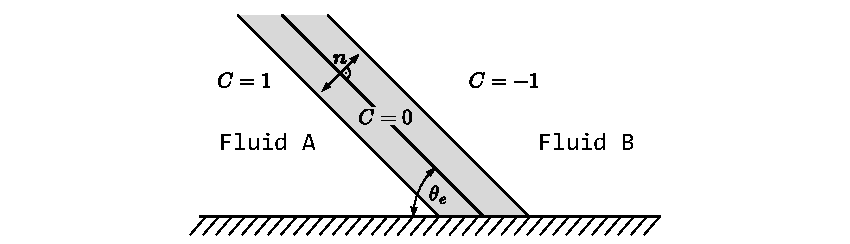
\includegraphics[width=.95\textwidth]{Pictures/DiffusiveInterface.pdf}
    \caption{Schematische Darstellung eines Diffusiven Interfaces}
    \label{fig: DiffusiveInteraface}
\end{figure}
In Abbildung \ref{fig: DiffusiveInteraface} ist die Kontakilinie eines Diffusiven interfaces dargestellt. Der Graue bereich ist der transitionsbereich des Ordnungsparameters und damit der Stoffgrößen. Innerhalb dieses Bereichs koexistieren beide Fluide mit ihren jeweiligen Dichten und viskositäten. Im Gleichgewichtszustand kann das Profil von $C$ normal zum Interface ermittelt werden, in dem die freie Energie (Gleichung \ref{eq: chempotentialMIXING_pahseFieldMethod})minimiert wird \cite{cai2015NumericalSimulationWetting}. Dies führt dann zu einer Beschreibung des Ordnungsparameters normal zum Interface mit
\begin{equation}
    \label{eq: InterfactialNormalDirProfile}
    C(n) = \tanh\left(\frac{n}{\sqrt{2}\epsilon}\right).
\end{equation}
Darin ist $n$ die normale auf dem Interface. Im gleichgewicht bleibt die Dicke des diffusen Interfaces gleich in einem Bereich von $3/\sqrt{2}\epsilon$ gilt für den Ordnungsparameter $-0.9\leq C\leq0.9$. Ebenfalls im Falle des Gleichgewichts, gleicht die Oberflächenspannung dem integral der freien energiedichte am Interface, woraus eine Beschreibung für die Oberflächenspannung abgeleitet werden kann \cite{jacqmin2000ContactlineDynamicsDiffuse}. 
\begin{equation}
\label{eq: surfacetensionEqui}
    \sigma = \int_{-\infty}^{\infty}\lambda\left( \frac{dC}{dn}  \right)^{2}= \frac{2\sqrt{2}}{3} \frac{\lambda}{\epsilon}
\end{equation}





\subsection{Wall Energy}






Jaqcmin \cite{jacqmin1999CalculationTwoPhaseNavier} postulierte eine Wandenergie der Form
\begin{equation}
    F_{\mathrm{w}}=\int \sigma g(C)dA, 
\end{equation}
womit die Wandenergie nur noch eine Funktion abhängig von der Fluidzusammensetzung direkt an der Wand abhängig ist. Die resultierende natürliche Phasenfeld Randbedingung mit lokalem thermischen Gleichgewicht ist gegeben mit
\begin{equation}
    \label{eq: BCfWall}
    \lambda \frac{\partial C}{\partial n_{\partial \Omega}} + f'_{\mathrm{w}}(C) =0.
\end{equation}
Mit $n_{\partial \Omega}$ als normalenrichtung auf der Wand (vgl. \ref{fig: DiffusiveInteraface}).
Die normalenrichtung zum interface kann mit der wandnormale und wand tangentiale Richtung auf der Wand beschrieben werden. 
\begin{equation}
    \label{eq: InterfaceNormal}
    n=n_{\partial\Omega}\cos{(\theta_{\mathrm{e}})}+\tau_{\partial\Omega}\sin{(\theta_{\mathrm{e}})}.
\end{equation}
Anschließend kann für den ersten Term aus Gleichung \ref{eq: BCfWall} mit den Gleichungen \ref{eq: InterfaceNormal}, \ref{eq: InterfactialNormalDirProfile} und \ref{eq: surfacetensionEqui} wie folgt erstellt werden
\begin{equation}
    \lambda\frac{\partial C}{\partial n_{\partial\Omega}} =\underbrace{\frac{3}{4}\sigma\left(1-C^2\right)\cos\theta_{\mathrm{e}}}_{=:-f'_\mathrm{w}(C)}.
\end{equation}
Daraus lässt sich eine Funktion für die Wandenergiedichte nach Integration ableiten\cite{jacqmin2000ContactlineDynamicsDiffuse}\cite{holzinger2021DirectNumericalSimulation}.
\begin{equation}
    f_{\mathrm{w}}(C)=-\sigma \cos\theta_e \frac{C(3-C^2)}{4} + \frac{\sigma_{S_L}+ \sigma_{S_V}}{2}
\end{equation}
Ist nur eine der Phasen anwesend, gibt diese Gleichung auch nur die jeweilige Oberflächenspannung zurück. Yue et al. \cite{yue2011WallEnergyRelaxation} weißt jedoch darauf hin, dass diese Beschreibung der Wandenergie für Gleichgewichtskontaktwinkel nahe $0^{\circ}$ oder $180^{\circ}$ nur schwer zu reproduzieren ist und das Modell nicht in der Lage ist precursor films zu handhaben. 



\section{Cahn-Hillard Navier Stokes Equations}
Die gekoppelten Cahn-Hillard Navier Stokes Gleichungen sind gegeben mit
\begin{align}
    \partial_t C + \nabla \cdot \left( C \mathbf{u} \right) &= -\nabla \cdot \mathbf{J} \\
    \nabla \cdot \mathbf{u} &= 0 \\
    \label{eq: NSEChanged}
    \partial_t(\rho \mathbf{u}) + \nabla \cdot (\rho \mathbf{u}\mathbf{u})&= -\nabla \tilde{p} + \nabla \mathbf{\tau} - \nabla \cdot(\mathbf{u}\mathbf{J})-\phi\nabla C + \mathbf{f}_{\mathrm{b}}
\end{align}

Darin ist $\tilde{p}$ ein modifizierter Druck, der aus dem Korteweg tensor entsteht, um die Kapillarität zu berücksichtigen. Die Annahme eines Newtonschen Fluids gilt $\mathbf{\tau} = 2\mu \mathrm{dev}\mathbf{D}$ mit $\mathbf{D} = 1/2[\nabla \mathbf{u}+(\nabla \mathbf{u})^{\mathrm{T}}]$ als Deformationstensor. Weiter ist die Dichte $\rho$ und viskosität $\mu$ volumetrisch gemittelt mit 
\begin{equation}
    \rho = \frac{1 + C}{2} \rho_1 +\frac{1 + C}{2} \rho_2.
\end{equation} 
Darin sind die suffixe $1$ und $2$ Markierungen für die jeweiligen Phasen. Die Viskosität wird analog berechnet. Der Term $- \nabla \cdot(\mathbf{u}\mathbf{J})$ ist notwendig, um die thermische consistenz zu gewährleisten \cite{ding2007DiffuseInterfaceModel}. $\mathbf{J}$ ist der phase-field flux und nach Landau und Lifshitz \todo{cite} gilt $\mathbf{J} = -M\nabla \phi$ 